\section{Schéma de synthèse}
\label{secSchemaConversion}

La figure~\ref{figChaineConversion} compare les trois chaînes de
conversion rencontrées sur la cellule : le PFC200 (déjà vu, un seul
niveau), puis le M221 et la baie CS9 (deux niveaux, avec un bloc
fonctionnel de conversion).

\begin{figure}[h]
    \centering
    \resizebox{\linewidth}{!}{%
    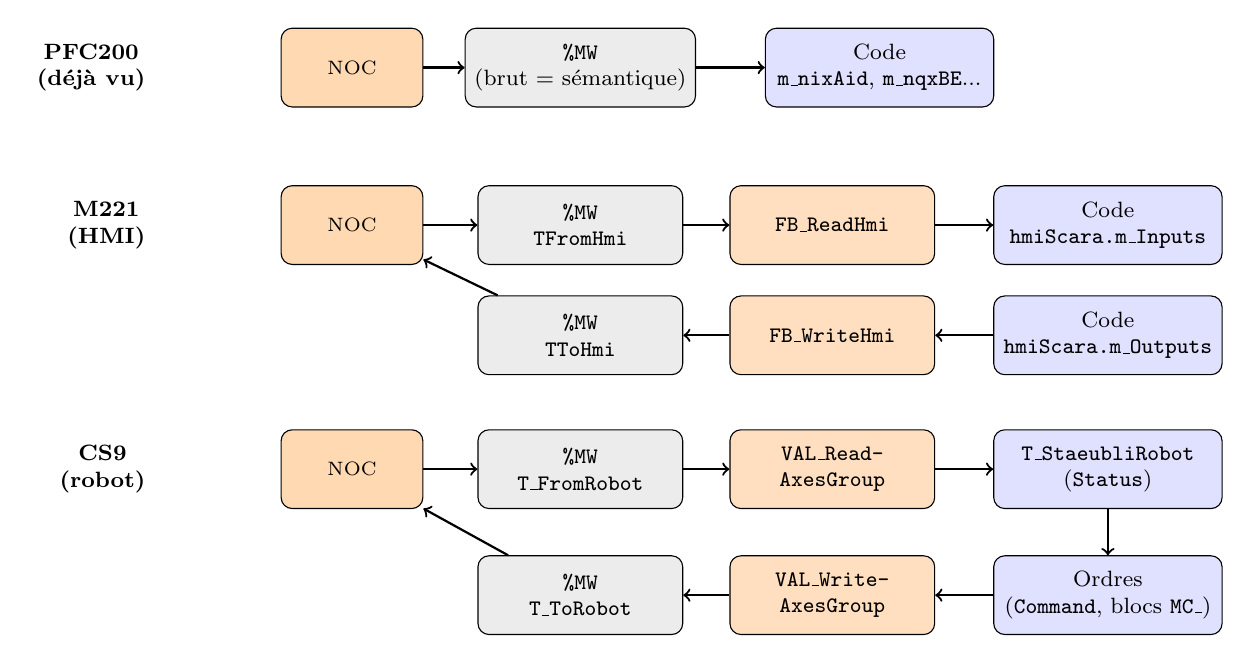
\begin{tikzpicture}[
        brut/.style = {draw, rounded corners, fill=gray!15, minimum width=2.6cm,
                        minimum height=1cm, align=center, font=\footnotesize},
        fb/.style = {draw, rounded corners, fill=orange!25, minimum width=2.6cm,
                        minimum height=1cm, align=center, font=\footnotesize},
        sem/.style = {draw, rounded corners, fill=blue!12, minimum width=2.9cm,
                        minimum height=1cm, align=center, font=\footnotesize},
        noc/.style = {draw, rounded corners, fill=orange!30, minimum width=1.8cm,
                        minimum height=1cm, align=center, font=\scriptsize},
        lien/.style = {thick, ->},
        rowlabel/.style = {font=\bfseries\footnotesize, anchor=east, align=center},
        ]

        % --- Ligne 1 : PFC200 (rappel, un seul niveau) ---
        \node[rowlabel] (lbl1) at (-6.3, 4) {PFC200\\(déjà vu)};
        \node[noc]  (noc1)  at (-3.8, 4) {NOC};
        \node[brut] (mw1)   at (-0.9,   4) {\texttt{\%MW}\\(brut = sémantique)};
        \node[sem]  (code1) at ( 2.9, 4) {Code\\\texttt{m\_nixAid}, \texttt{m\_nqxBE}...};
        \draw[lien] (noc1) -- (mw1);
        \draw[lien] (mw1) -- (code1);

        % --- Ligne 2 : M221 (HMI) ---
        \node[rowlabel] (lbl2) at (-6.3, 2) {M221\\(HMI)};
        \node[noc]  (noc2)  at (-3.8, 2) {NOC};
        \node[brut] (mw2)   at (-0.9, 2) {\texttt{\%MW}\\\texttt{TFromHmi}};
        \node[fb]   (fb2)   at ( 2.3, 2) {\texttt{FB\_ReadHmi}};
        \node[sem]  (code2) at ( 5.8, 2) {Code\\\texttt{hmiScara.m\_Inputs}};
        \draw[lien] (noc2) -- (mw2);
        \draw[lien] (mw2) -- (fb2);
        \draw[lien] (fb2) -- (code2);

        \node[sem]  (code2b) at ( 5.8, 0.6) {Code\\\texttt{hmiScara.m\_Outputs}};
        \node[fb]   (fb2b)   at ( 2.3, 0.6) {\texttt{FB\_WriteHmi}};
        \node[brut] (mw2b)   at (-0.9, 0.6) {\texttt{\%MW}\\\texttt{TToHmi}};
        \draw[lien] (code2b) -- (fb2b);
        \draw[lien] (fb2b) -- (mw2b);
        \draw[lien] (mw2b) -- (noc2);

        % --- Ligne 3 : CS9 (robot) ---
        \node[rowlabel] (lbl3) at (-6.3, -1.1) {CS9\\(robot)};
        \node[noc]  (noc3)  at (-3.8, -1.1) {NOC};
        \node[brut] (mw3)   at (-0.9, -1.1) {\texttt{\%MW}\\\texttt{T\_FromRobot}};
        \node[fb]   (fb3)   at ( 2.3, -1.1) {\texttt{VAL\_Read-}\\\texttt{AxesGroup}};
        \node[sem]  (code3) at ( 5.8, -1.1) {\texttt{T\_StaeubliRobot}\\(\texttt{Status})};
        \draw[lien] (noc3) -- (mw3);
        \draw[lien] (mw3) -- (fb3);
        \draw[lien] (fb3) -- (code3);

        \node[sem]  (ordres) at ( 5.8, -2.7) {Ordres\\(\texttt{Command}, blocs \texttt{MC\_})};
        \node[fb]   (fb3b)   at ( 2.3, -2.7) {\texttt{VAL\_Write-}\\\texttt{AxesGroup}};
        \node[brut] (mw3b)   at (-0.9, -2.7) {\texttt{\%MW}\\\texttt{T\_ToRobot}};
        \draw[lien] (code3) -- (ordres);
        \draw[lien] (ordres) -- (fb3b);
        \draw[lien] (fb3b) -- (mw3b);
        \draw[lien] (mw3b) -- (noc3);

    \end{tikzpicture}}
    \caption{Chaîne de conversion NOC $\to$ mémoire $\to$ code applicatif, selon l'équipement}
    \label{figChaineConversion}
\end{figure}

\begin{UPSTIinfor}{Ce que montre ce schéma}
Sur les trois équipements, l'alias mémoire sur la zone \texttt{\%MW} reste
le point d'entrée/sortie unique. Ce qui change, c'est ce qu'il faut faire
\emph{après} cet alias : rien de plus pour le PFC200, un passage par un
bloc fonctionnel de conversion pour le M221 et pour la baie CS9. Dans ce
dernier cas, le même objet sémantique (\texttt{T\_StaeubliRobot}) sert à
la fois à \textbf{lire} l'état du robot et à \textbf{lui donner des
ordres} : c'est pour cela qu'il est passé en \texttt{VAR\_IN\_OUT} aux
deux blocs \texttt{VAL\_Read/WriteAxesGroup}, et non simplement en entrée
ou en sortie.
\end{UPSTIinfor}

\begin{UPSTIactivite}[4][Suivre une information le long de la chaîne][][][TD]
\UPSTIquestion{L'opérateur appuie sur le bouton-poussoir « J3 : Up » du
pupitre. En s'appuyant sur la figure~\ref{figChaineConversion}, citer
dans l'ordre les objets et blocs traversés par cette information, depuis
le coupleur \texttt{NOC\_ETHIP\_ROBOT} jusqu'au champ
\texttt{hmiScara.m\_Inputs.m\_nixJ3Up} lu par le programme applicatif.}
\UPSTIquadrillage{3}

\begin{UPSTIcorrectionP}{Corrigé}
Coupleur \texttt{NOC\_ETHIP\_ROBOT} (connexion avec le M221) $\to$ zone
\texttt{\%MW} image des données reçues du M221 $\to$ alias
\texttt{fromHmiScara} (type \texttt{TFromHmi}, octets bruts) $\to$ bloc
\texttt{FB\_ReadHmi} (instance \texttt{InstReadHmi}, paramètre
\texttt{fromHmi}) $\to$ objet sémantique \texttt{hmiScara} (type
\texttt{THmi}), champ \texttt{hmiScara.m\_Inputs.m\_nixJ3Up}.
\end{UPSTIcorrectionP}

\UPSTIquestion{Faire de même pour la position cartésienne du robot
affichée sur l'écran du pupitre : depuis la baie CS9 jusqu'au M221. Quel
objet sémantique sert de « pont » entre la chaîne du robot et celle de
l'IHM ?}
\UPSTIquadrillage{4}

\begin{UPSTIcorrectionP}{Corrigé}
Baie CS9 (serveur \texttt{uniVALplc}) $\to$ coupleur
\texttt{NOC\_ETHIP\_ROBOT} $\to$ zone \texttt{\%MW}, alias
\texttt{fromRobotScara} (\texttt{T\_FromRobot}) $\to$
\texttt{VAL\_ReadAxesGroup} (paramètre \texttt{IN}) $\to$
\texttt{staeubliRobotScara.Status.CartesianPos} (\texttt{T\_StaeubliRobot})
$\to$ \texttt{FB\_WriteHmi} (paramètre \texttt{AxesGroup}), qui construit
$\to$ \texttt{toHmiScara} (\texttt{TToHmi}, sortie \texttt{toHmi}) $\to$
zone \texttt{\%MW} $\to$ coupleur \texttt{NOC\_ETHIP\_ROBOT} $\to$ M221
(écran du pupitre).

L'objet « pont » est \texttt{staeubliRobotScara} (type
\texttt{T\_StaeubliRobot}) : mis à jour par \texttt{VAL\_ReadAxesGroup}, il
est transmis sur le paramètre \texttt{AxesGroup} des blocs
\texttt{FB\_ReadHmi}/\texttt{FB\_WriteHmi}, d'où l'ordre d'appel imposé
(après \texttt{VAL\_ReadAxesGroup}).
\end{UPSTIcorrectionP}
\end{UPSTIactivite}
